\clearpage
\section{Literature}

TODO: table with all keywords and search results

Literature to answer these questions will be gathered with the following procedure:
\begin{enumerate}
\item List search relevant search terms.
\item Find synonyms in a thesaurus.
\item Search literature on Google Scholar \cite{scholar}, Science Direct \cite{science-direct} and Papers with Code \cite{paperswithcode}. 
\item Select potential papers based on their title and abstract.
\item Check Google Scholar which cite the respective paper to see if a more recent version exists (forward citation).
\item Scan through paper references if a specific title seems relevant (backward citation), repeat from 4.
\end{enumerate}



\subsection{Automatic Road Defects Classification}

Preliminary literature review shows that there is a whole field about data driven road quality assessment. This field is driven by the fact that traditional methods of assessing road quality is costly, due requirement of specialized equipment. Researchers focuses on alternative forms to collect the data by cheaper methods, such as smartphones and sensor boxes. In current literature we identified the following \textit{subfields} based on the type of data that is used:

\begin{enumerate}
\item Road surface defects: based on image data (e.g. cracks).
\item Roughness evaluation: based on accelerometer / gyroscope (e.g. IRI).
\item Noise labelling: based on microphones.
\end{enumerate}

\begin{figure}[h!]
\begin{center}
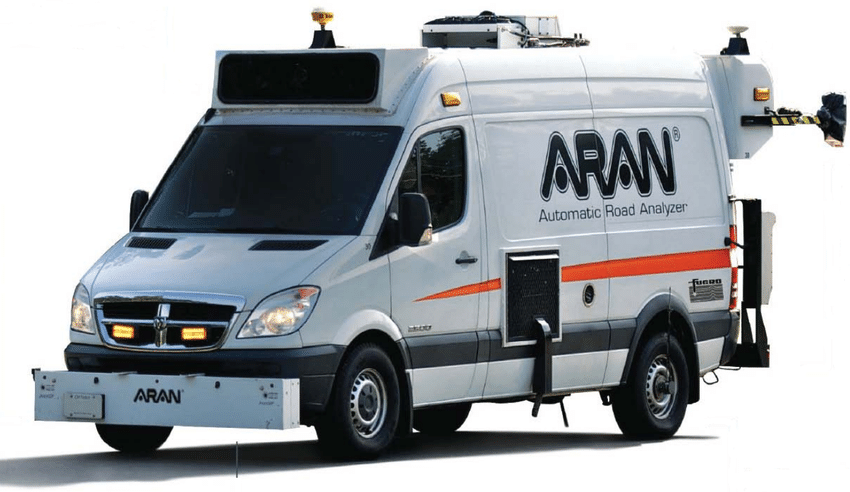
\includegraphics[height=5cm,keepaspectratio]{images/2_literature/aran.png}
\end{center}
\caption{Automatic Road Analyzer (ARAN) is specialized vehicle to gather data about the road surface \cite{Gupta2020}.}
\end{figure}

\subsubsection{Road surface defects}
Road surface defects or crack detection is a field trying to automatically classify damages based on image data. Usually the source of these images are smartphones. Additionally, there is also research performed using blackboxes (dashcams) and Kinect, where the latter is also able to measure depth. Research evolved from pictures taken from a top-down view, to front-faced view to support gathering data while driving.

In \authorref{Jahanshahi2012} the authors uses a Kinect sensor to collect image and depth data. Recording of the road has been performed from a top-faced view. The authors classify cracks, potholes and patches with accuracy scores of respective 78\%, 92\% and 90\%. By including depth measure, the problem is relatively trivial as classification is done by checking if the depth is greater than some threshold. 

\authorref{Zhang2016} proposes the first model (to their knowledge) which uses deep learning to detect road cracks. Their data has been collected by smartphones, although not mentioned explicitly, it seems their data has been collected from top-faced view and from deliberate pictures of a known defect. Related is \authorref{Zhang2017} where the authors use 3D pavement images and deep-learning network to classify road cracks. Their research is focused on acquiring pixel-level accuracy, with the aim that the model is able to tell the size and dimensions of the crack.

\authorref{Chatterjee2018} perform road crack detection on cycle roads in Germany. Their data has been collected from a front-faced view. Extensive feature extraction is performed with various computer vision based algorithms before making classifications with machine learning models. 

\authorref{Maeda2018} researched the possibilities of road damage classification by using smartphone images. Data was collected conventional smartphone holder for cars with a front-faced view while driving. They extensively collect data about Japanese roads and publishes their data and their trained model. This is also the first paper which makes distinctions between more types of road damages, such as fading line markings and distinction between lateral / longitudal cracks. The research is continued in \authorref{Arya2020-transfer}, where additional data is collected in Czech Republic and India. With the aim to see if their model is able to transfer learn on this new data. In order to further improve the published model, \authorref{Maeda2020} uses a generative adversial network to augment more data and retrain the model. Finally, a competition is held with their collected data \cite{Arya2020-competition}. The goal is to push the state of art of road damage detection forward. The competition consisted of two challenges: 1) classification (what kind of damage) and 2) detection (where is the damage). This competition yielded a model with an average F1 score of 0.67 for all classes. Greatly improving the original model, which yielded at best a F1 of 0.40 for only a single type of damage.

Besides making classifications, there has also been research focusing on segmenting the damages into crack and non-crack parts. \authorref{Dung2018} uses a fully convolutional neural network and \authorref{Bang2019} uses a encoder-decoder network.


\subsubsection{Roughness evaluation}
A different research field is centered around measuring the road roughness. Which is defined as the deviation of the surface from the true planar surface. This deviation affects vehicle dynamics and ride quality. Two methods to classify the roughness of a profile are the International Roughness Index (IRI) \cite{Sayers1986} and the International Standards Organisation (ISO) \cite{ISO8608} classification. There are various methods for measuring the profile data, typically used by road maintenance are inertial profilers. This is a device which scans the surface of the pavement with lasers to measure the distance, example of this is the Automatic Road Analyzers (ARAN) vehicle.

Research is focused on replacing these expensive devices with accelerometers, often those found in smartphones \cite{Hanson2014,Buttlar2014,Gupta2020}. Measuring the profile is done by filtering out the vertical accelerations and calculate the roughness accordingly to the IRI or ISO specification. Additionally, using the accelerometer it is also possible to identify potholes, bumps and patches \cite{Lekshmipathy2020}. 

Limitation of this method is that the accelerometers need to be calibrated, which is also deeper described in \cite{Gupta2020}. \authorref{Jeong2020} therefore argue that requirement of calibration hinders the widespread use of the technology. They propose a novel method using a convolutional neural network to eliminate the requirement of calibration.


\subsubsection{Noise labelling}
Quality of the road surface influences noise and vibrations emissions caused by the interaction between the tires and the road. In the EU, member states are required to publish noise maps for roads every five years \cite{EU2002}. Monitoring can be done with a vehicle equipped with a Close Proximity (CPX) trailer. This devices measures the emitted sounds from a reference tire.

\begin{figure}[ht]
\begin{center}
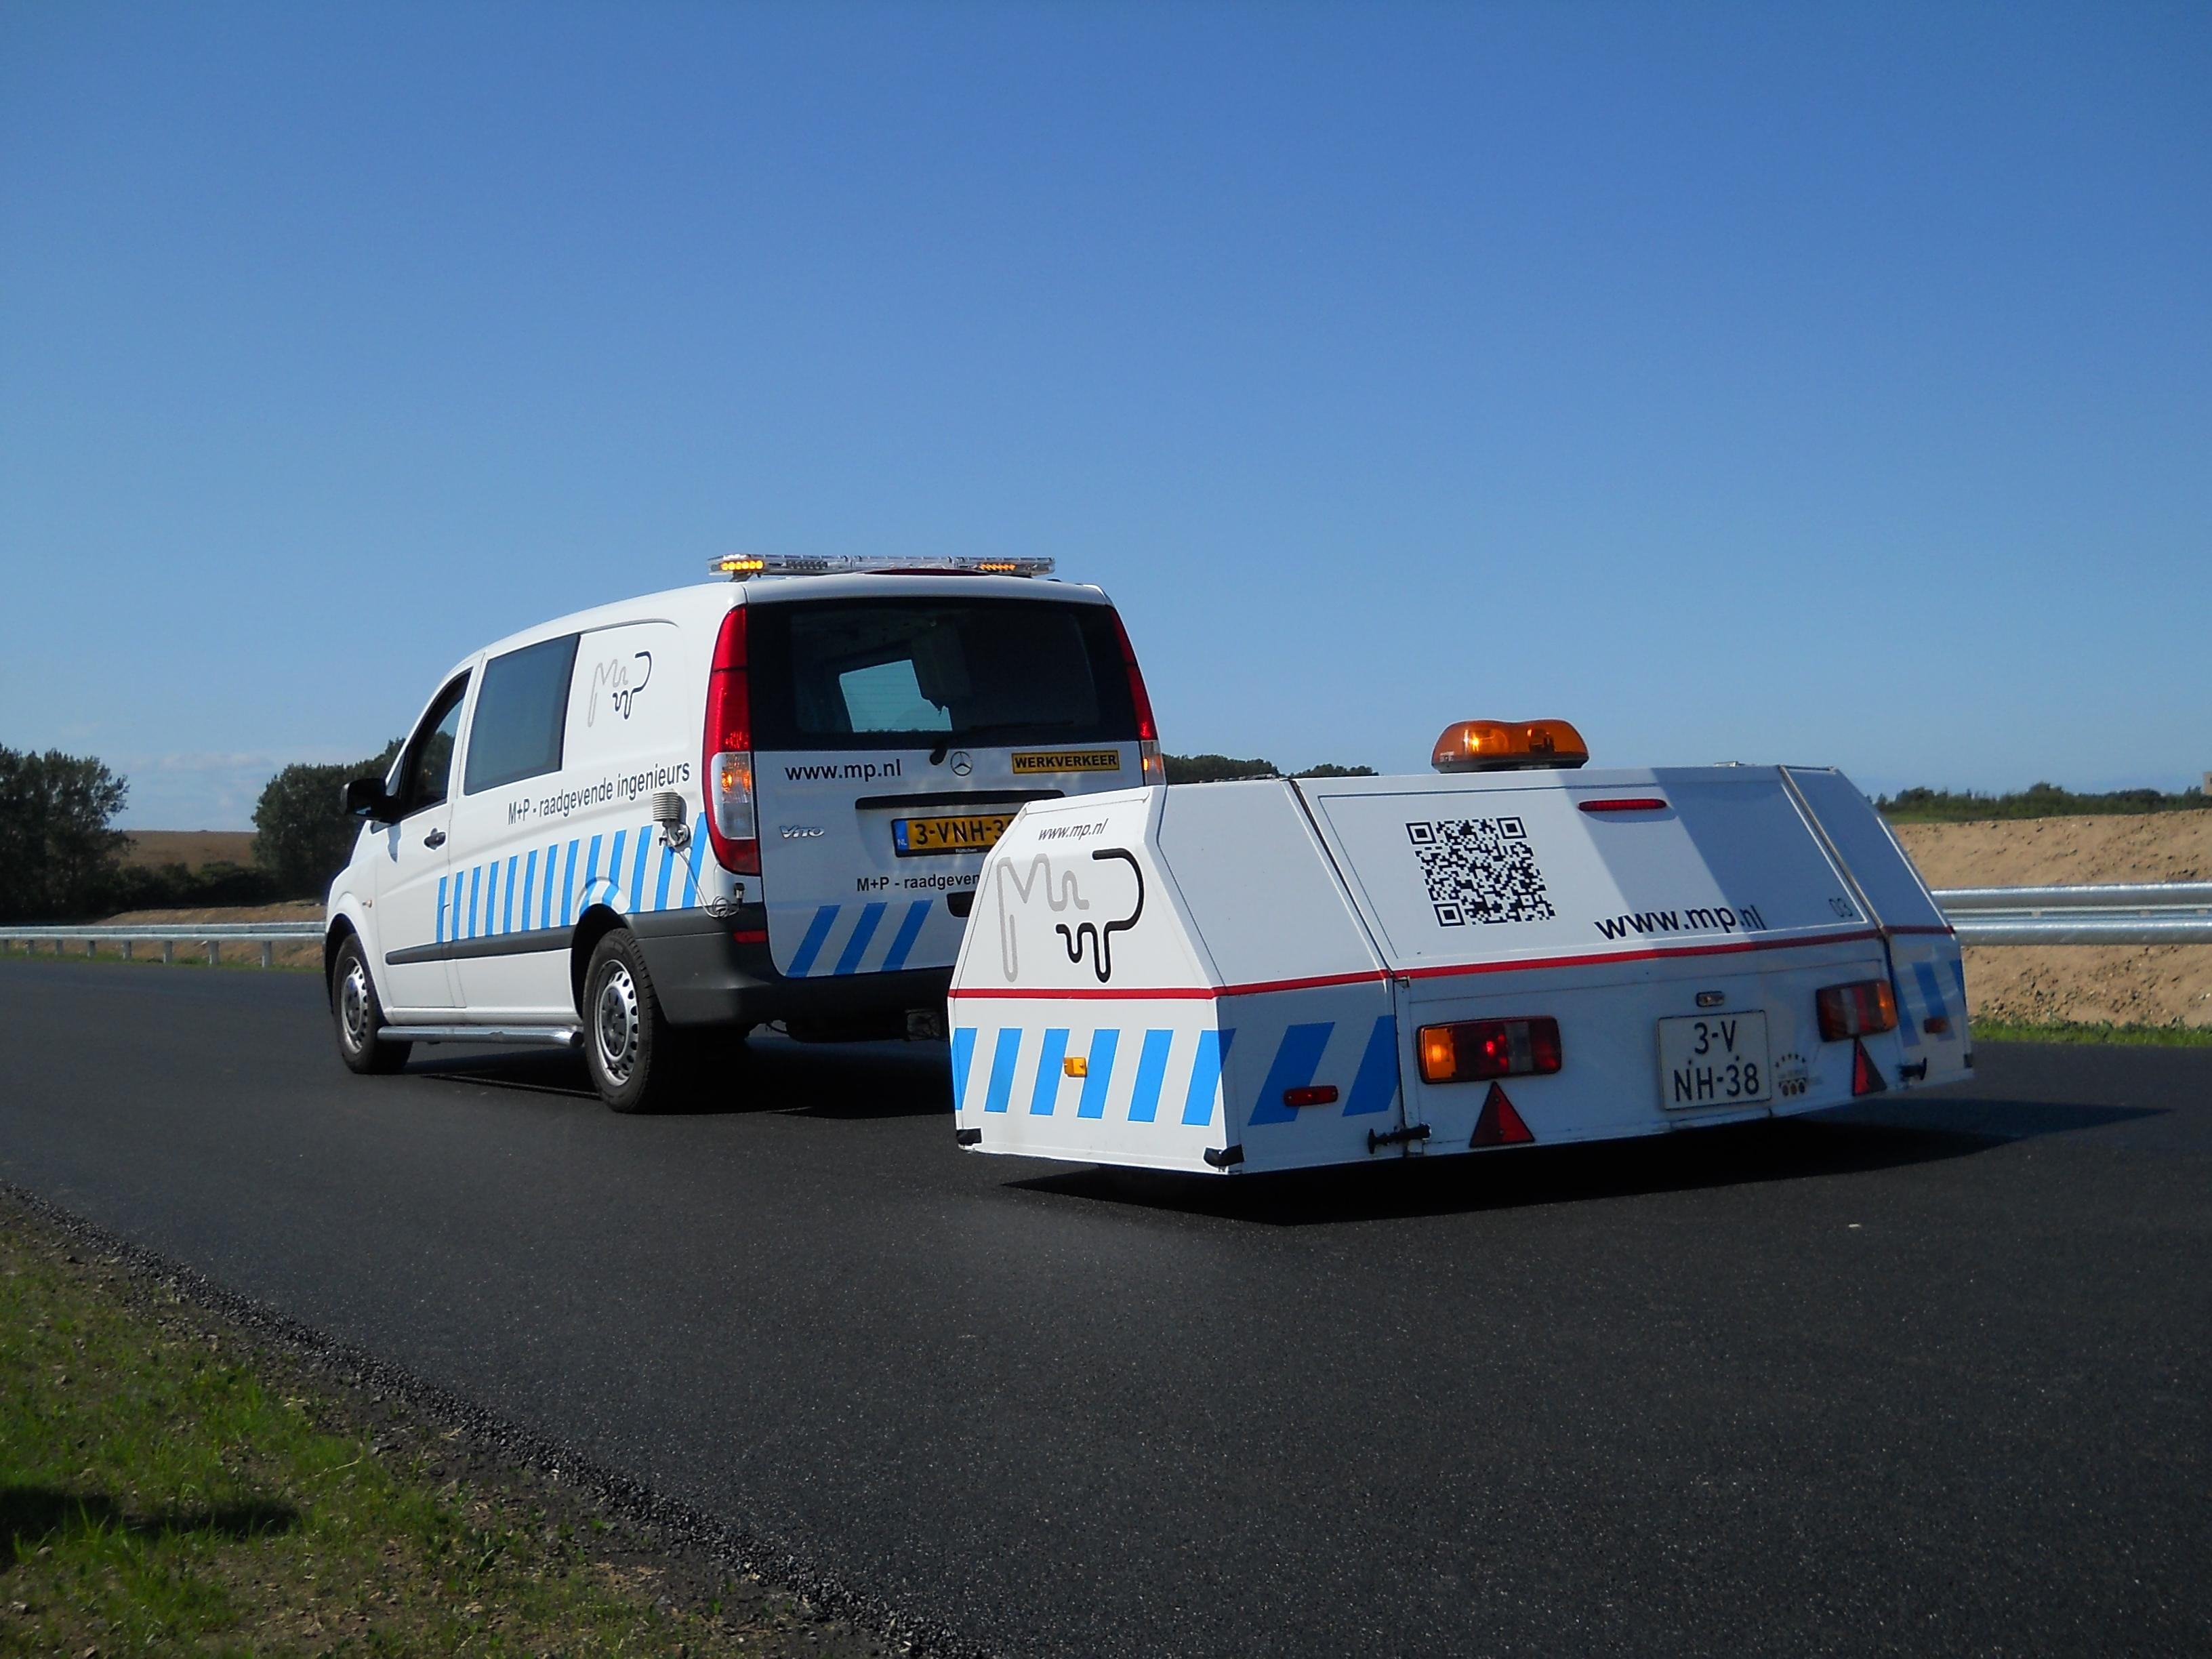
\includegraphics[height=5cm,keepaspectratio]{images/2_literature/cpx-trailer.jpg}
\end{center}
\caption{Close Proximity (CPX) trailer measures the sounds emitted by reference tyre \cite{MP2020}.}
\end{figure}

\authorref{Hauwermeiren2019} try to replicate the results of CPX measurements by using a sensor box containing a microphone. This microphone is located inside the trunk of the car. The authors were able to accurately estimate the road texture. However the with main limitation is that the data was collected under good conditions, such as no background radio or talking. This research is later continued, where the authors use multiple vehicles and more realistic driving conditions. They found that below 1600 Hz, their results differ from CPX less than the difference between bi-annually repeated measurements, indicating it is possible to perform this measurement using microphones \cite{Hauwermeiren2021}.


\subsubsection{Conclusion}
Automatic classification of road defects have been extensively researched. Main topic of interest is the usage of low-cost devices such as smartphones to collect the data. From the literature we find that only the following types of defects are classified: cracks, patches, holes and faded line markings. Raveling, rutting and skewed signs haven't been researched yet to my knowledge. From the field of classifying road defects we can draw a lot of knowledge to use for my thesis. Especially this is useful when to model the right representations of the data to use for multimodal machine learning.


% ********************************************************************************
% ********************************************************************************
% ********************************************************************************

\subsection{Object Detection}

\textit{TODO: introduce topic}

State of the art visual road defects detection rely on object detection. Object detection is the combination of classifying and locating the object. The output of the model is the detected class and the bounding box where that object is detected. Within a single image there can be one or multiple defects, sometimes from different types. With object detection it is possible to locate all these different instances. Object detection is well researched topic. The most commonly referred models are known as R-CNN, Fast R-CNN, Faster R-CNN and YOLO.


\subsubsection{R-CNN}
A naive approach to solve the problem of localizing objects is to slide a window over the image, and for each window perform classification. However the problem with this approach is that objects may have different location, sizes and aspect ratios. To make this work, an infinite possibility of regions need to be computed. 

\authorref{Girshick2013} solves this problem by proposing a model called Regions with CNN (R-CNN). Their approach is to extract 2000 regions using a region proposal algorithm (in paper they use selective search). For each region they use a CNN to extract features and SVM to make the classification. 

\begin{figure}[ht]
\begin{center}
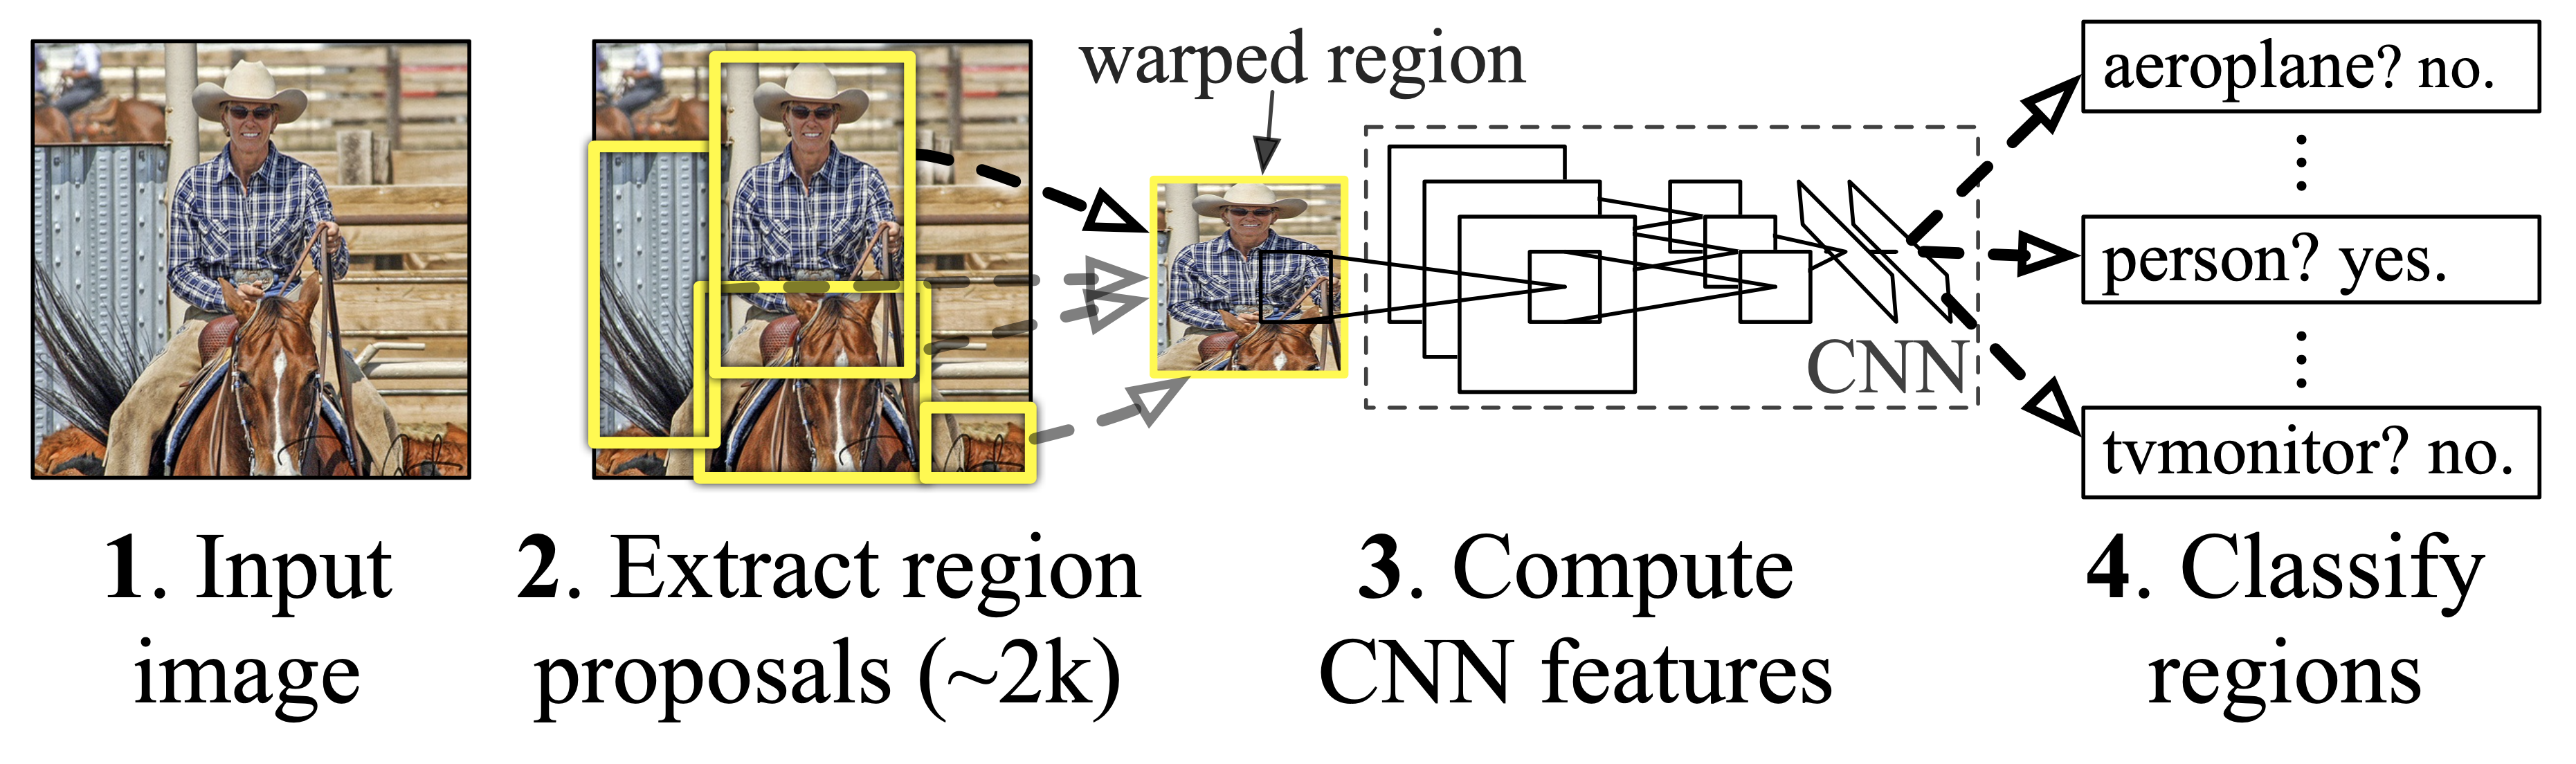
\includegraphics[height=2cm,keepaspectratio]{images/2_literature/r-cnn.png}
\end{center}
\caption{R-CNN: Object detection overview \cite{Girshick2013}.}
\end{figure}

\subsubsection{Fast R-CNN}
Drawback of the method above has some drawbacks. Mainly it is slow because it performs a CNN for each of the 2000 object proposals. The author\authorref{Girshick2015} continued its work to solve this problem. With the new proposed model called Fast R-CNN. This novel model can detect object in an image in 2 seconds, whereas the original R-CNN takes about 50 seconds per image.

Instead of feeding each of the proposed regions to the CNN, the Fast R-CNN takes as input the entire input image and proposed regions. From the output, regions of interests are identified and are fed into fully connected layers to output the class and location of the object. 

\begin{figure}[ht]
\begin{center}
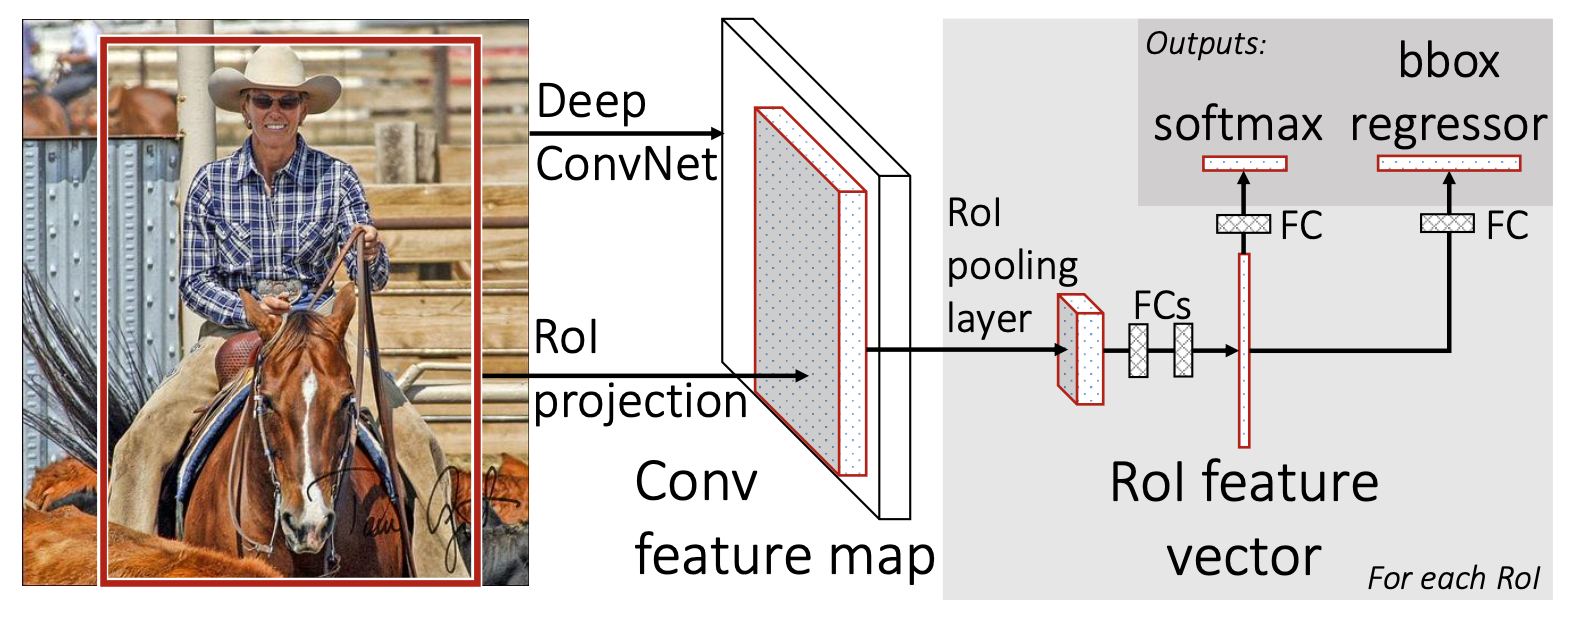
\includegraphics[height=2cm,keepaspectratio]{images/2_literature/fast-r-cnn.png}
\end{center}
\caption{Fast R-CNN: Object detection overview \cite{Girshick2013}.}
\end{figure}

\subsubsection{Faster R-CNN}
Although Fast R-CNN is significantly quicker to detect objects, it still takes about 2 seconds to localize the object. The bottleneck is the region proposal algorithm, which is implemented on the CPU. Improvements over the used selective search were researched. However, \authorref{Ren2015} argued that it would be interesting to implement a model which combines region proposal and object detection. Their model was called Faster R-CNN and is able to process an image in 200 milliseconds. 

Faster R-CNN consists of two modules. The first module is a deep fully convolutional network which proposes regions, known as Region Proposal Network (RPN). The RPN takes an image as input and outputs a set of object proposals, each with an \textit{objectness score} (measurement if something is an object or background). This output is fed into the second module, which is the Fast R-CNN object detector. 

The unified model has several advantages over the Fast R-CNN model. Because the region proposal are generated within the network, the model can be trained end-to-end. Making usage easier and requires less resources. Additionally, this allows the region proposals to be tuned according to the detection task.


\begin{figure}[ht]
\begin{center}
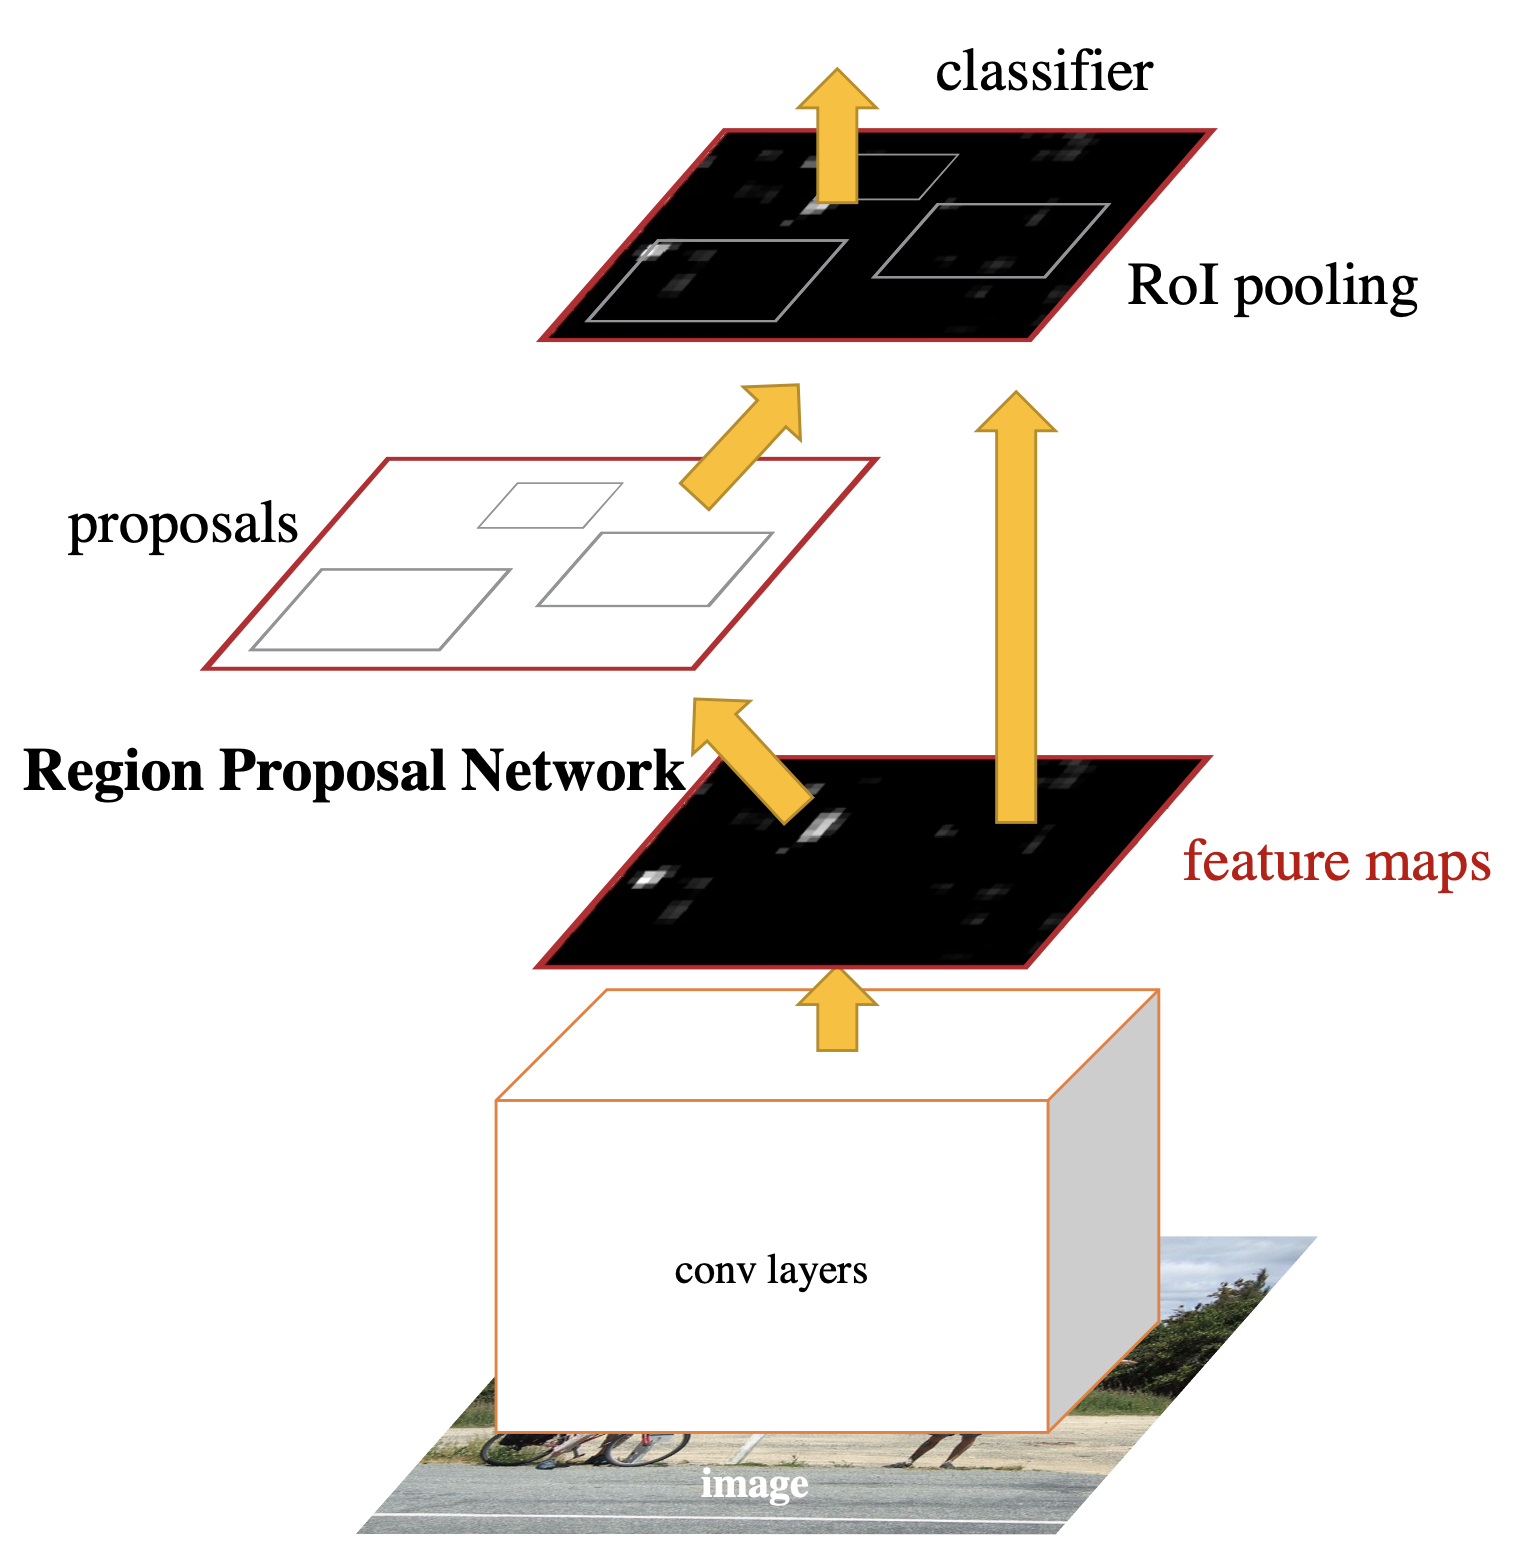
\includegraphics[height=5cm,keepaspectratio]{images/2_literature/faster-r-cnn.png}
\end{center}
\caption{Faster R-CNN: Object detection overview \cite{Ren2015}.}
\end{figure}


\subsubsection{YOLO}
The previous detectors all use regions to localize an object. The models look at parts of the image with high probability of containing an object. YOLO has a different architecture by looking at the complete image. A single neural network predicts bounding boxes and class probabilities in one evaluation. Using the system, you only look once (YOLO) at an image to see what objects it contains \cite{Redmon2016}.

YOLO as several benefits. First of all is that YOLO is extremely fast. Due the new architecture, it doesn't require a complex pipeline and can be trained end-to-end. Secondly, unlike previous models, YOLO reasons globally about the image. Most mistakes from top detector Fast R-CNN are due mistaking background for an object. YOLO makes less than half the number of background errors compared to Fast R-CNN. Finally, YOLO learns generalizable representations of objects. When trained on natural images and tested on art-work, YOLO outperforms top detectors such as R-CNN. 

YOLO does lag behind state-of-the-art detectors in accuracy. Although it can quickly detect objects, its struggles to precisely localize some objects, especially small ones. 

YOLO works by taking an image and split it into an SxS grid. Each grid predicts B bounding boxes and confidence scores for those boxes. These scores reflect how confident the model is that the box contains an object. The model outputs for each bounding box 5 predictions, the location (x, y), size (w, h) and confidence score. Additionally, each grid cell also predicts C conditional class probabilities. 

\begin{figure}[ht]
\begin{center}
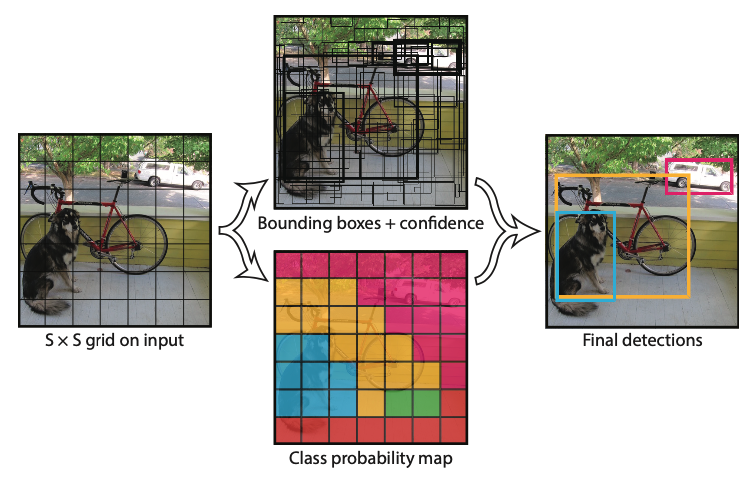
\includegraphics[width=10cm,keepaspectratio]{images/2_literature/yolo.png}
\end{center}
\caption{You Ony Look Once (YOLO) detector model \cite{Redmon2016}.}
\end{figure}


\subsubsection{YOLOv2}
The authors of YOLO continued their work and introduce two new detectors YOLOv2 and YOLO9000 \cite{Redmon2017}. They argue that current object detection datasets are limited (hundred thousand images) compared to datasets used for classification and tagging (millions of images with thousands of categories). They propose a novel method to harness large amount classification data and use it to expand current detection systems. Using this method they develop YOLO9000, a real-time object detector that can detect over 9000 categories. To do so, they first improve the base YOLO detection system to produce YOLOv2. 

YOLO suffers from various shortcomings relative to state-of-the-art detection systems. YOLO makes significantly number of localization errors compared to Fast R-CNN. Better performance often comes from training larger networks or ensambling networks together, instead the authors opt to simplify the network and introduce several architectural changes. In short, most improvements stem by applying state-of-the-art deep learning techniques, for details see \cite{Redmon2017}.  Below is shown an comparison of accuracy and speed between various detectors to demonstrate the effects.


\begin{figure}[ht]
\begin{center}
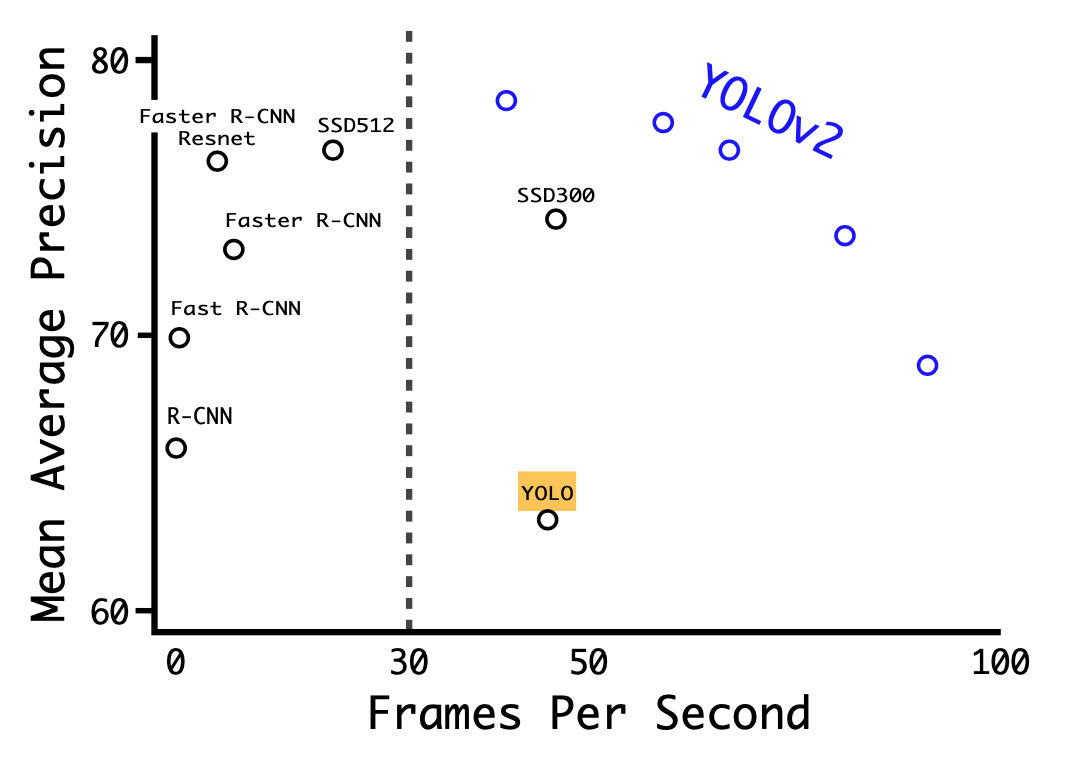
\includegraphics[width=10cm,keepaspectratio]{images/2_literature/yolov2-performance.png}
\end{center}
\caption{YOLOv2 accuracy and speed comparison on VOC 2007 \cite{Redmon2017}.}
\end{figure}

\subsubsection{YOLOv3}
YOLOv3 is another improved version of YOLO by the same authors \cite{Redmon2018}. It uses a new base model which is a bit slower but more accuracte. YOLOv3 predicts boxes at 3 different scales, based on the idea of Feature Pyramid Network \cite{Lin2017}. This allows the model to learn objects at different scales. Improving the performance of detecting smaller objects. Additionally, YOLOv3 performs multilabel classification instead of earlier used softmax.  Softmax asummes that labels are mutually exclusive, however it should be possible to classify an object as both woman and person. 


\begin{figure}[ht]
\begin{center}
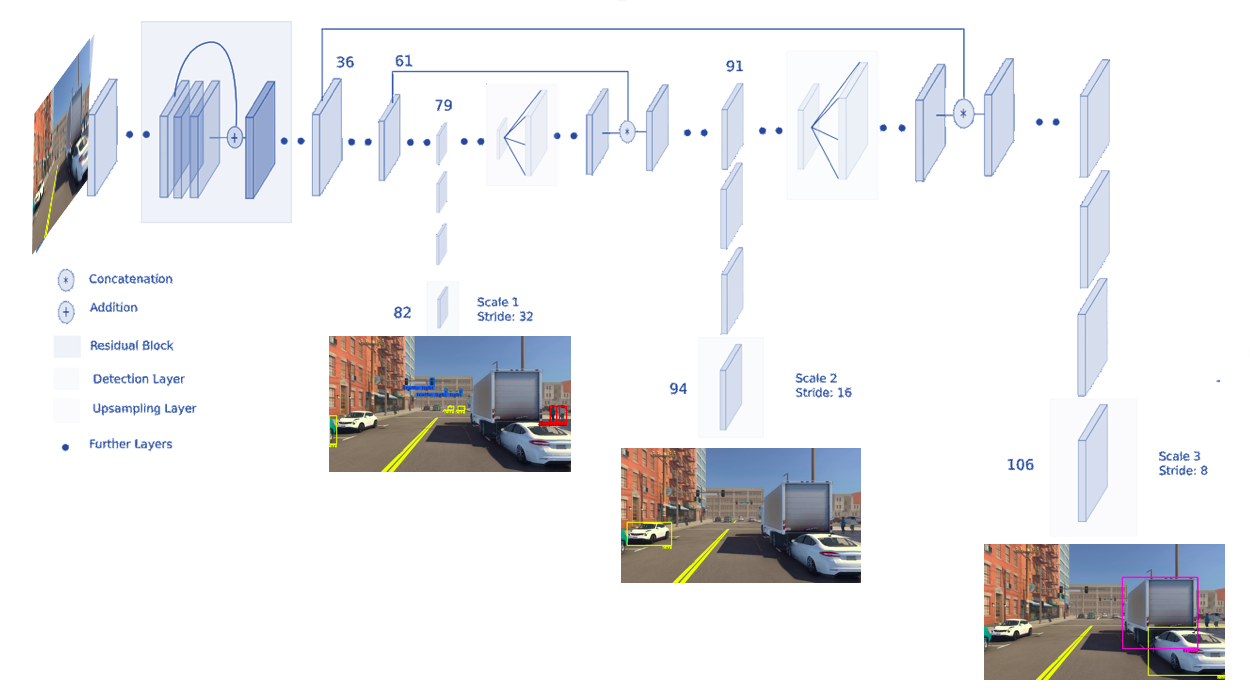
\includegraphics[width=14cm,keepaspectratio]{images/2_literature/yolov3-architecture.png}
\end{center}
\caption{YOLOv3 network architecture \cite{Dulepet2020}. Note that based on the output scale, the model detects objects of different sizes.}
\end{figure}


\subsubsection{YOLOv4}

YOLOv4 is the successor of YOLOv3. Unlike earlier models, YOLOv4 is developed by other authors \cite{Bochkovskiy2020}. In their paper the authors explore various deep learning techniques to improve the performance of YOLO, some deriving from earlier research, as well some novel techniques. The results is an improvement of 10\% accuraccy and about 12\% increase in speed.

One of these novel techniques is named Mosaic. It is a data augmentation method that mixes 4 training images. Thus 4 contexts are mixed. This allows detection of objects outside their normal context. In addition, batch normalization calculates statistics from 4 different images. Reducing the need for large mini-batch sizes.

Another novel technique is Self-Adversarial Training (SAT). This is also a data augmentation technique that operates in 2 stages. In the first stage, the network modifies the image instead of the weights. Thereby performing an adversarial attack on itself. In the second stage, the network is trained to detect an object on this modified image.


\subsubsection{YOLOv5}

Currently, there is no paper released on YOLOv5. At this time, it seems that YOLOv5 is still under active development \cite{Jocher2021}. Nevertheless, it has already been included in research \cite{Arya2020-competition}.


\subsubsection{Detection Transformers}

A complete different approach to object detection is DEtection TRansformers (DETR) \cite{Carion2020}. Transformers are deep learning architecture that recently gained popularity. They rely on powerful mechanism called attention, which enables the model to focus on certain parts of their input. 

\textit{TODO: To research further}


\subsubsection{Conclusion}



% ********************************************************************************
% ********************************************************************************
% ********************************************************************************


\subsection{Multimodal Machine Learning}

We experience the world as multimodal: we see objects, feel vibrations and hear sounds. Modality refers to the way in which something happens or is experienced. A research problem is characterized as multimodal when it includes multiple of such modalities \cite{Baltrusaitis2017}. Commonly referred example of an everyday multimodal experience is the McGurk effect \cite{McGurk1976}. This is the perception between hearing and vision in speech: when we hear the syllable /ba/ while watching the lips of someone saying /ga/, we perceive it as /da/. 

Multimodal research has a long history from audio-visual speech recognition to more recent interest due deep learning \cite{Ngiam2011}. It has been proven that multimodal learning algorithms performs really well on various tasks, such as (audio-visual) speech recognition \cite{Noda2014}, image sentence matching \cite{Ma2015} and RGB-D object recognition \cite{Eitel2015,Xu2017,Sindagi2019}.

\authorref{Baltrusaitis2017} identified five challenges dealing with multimodal machine learning:
\begin{enumerate}
\item \textbf{Representation}: how to represent and summarize multimodal data to exploit the complementary and redundancy of multiple modalities. Distinction is made between \textit{joint representation} - which combines unimodal signals in the same space, and \textit{coordinated representation} - which processes unimodal signals separately, but enforces similarity constraints. See figure \ref{fig:structure-joint-coordinated} below for an illustration.
\item \textbf{Translation}: how to translate data from one modality to another. For example, given an image the task is to give a caption to describe the image.
\item \textbf{Alignment}: how to identify direct relations between (sub)elements from multiple modalities. For example, given an image and a caption, find the area in the image describing the caption.
\item \textbf{Fusion}: how and when to fuse / join information from multiple modalities. Historically the original topics of multimodal machine learning, with emphasize given on early-, hybrid- and late-fusion.
\item \textbf{Co-learning}: how to transfer knowledge between modalities. For example by exploiting knowledge of a rich modality, to aid modelling of a less describing modality.
\end{enumerate}

\begin{figure}[ht]
\begin{center}
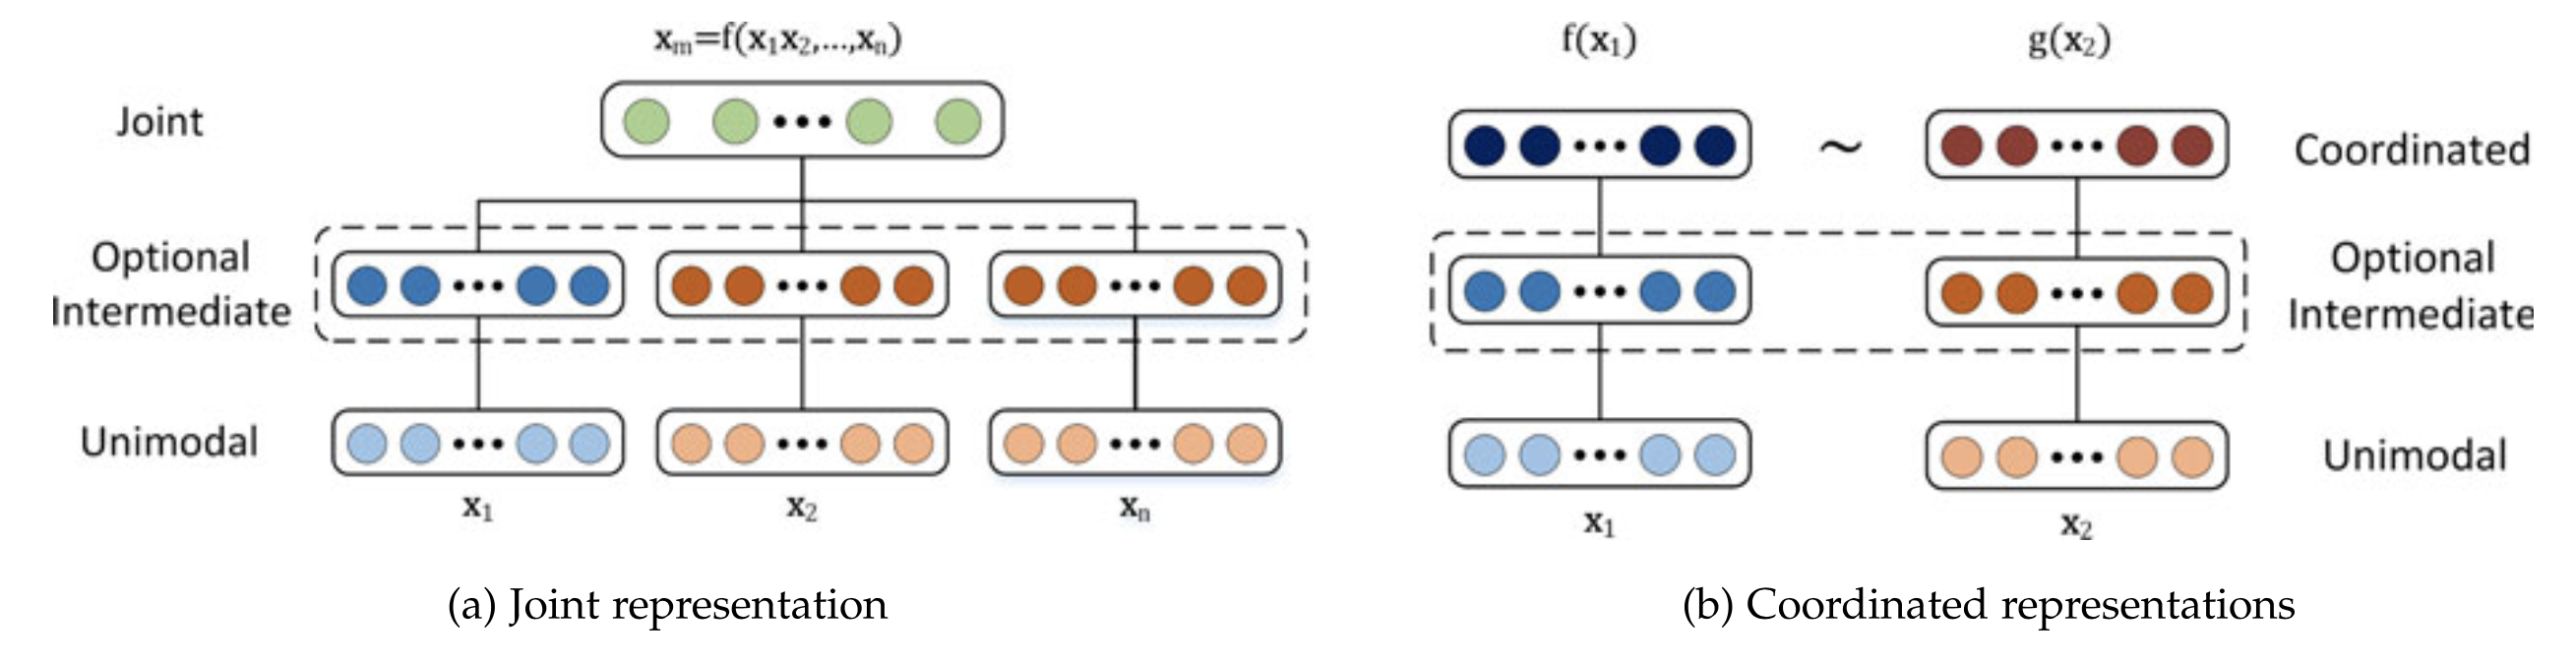
\includegraphics[width=\textwidth,keepaspectratio]{images/2_literature/joint-vs-coordinated-representations.png}
\end{center}
\caption{Structure of joint and coordinated representation \cite{Baltrusaitis2017}}
\label{fig:structure-joint-coordinated}
\end{figure}

To my knowledge there hasn't been any research performed on multimodal fusion on road defects. In the broader sense, multimodal fusion has been applied to detect damages. Examples of which are: combining audio-visual data to detect conveyor belt damages \cite{Che2021}, gearbox fault detection based on vibrations and acoustic signals \cite{Li2016}. See \cite{Olivan2018} for more examples of data fusion in industry.

Further exploratory research shows that visual and accelerometer (IMU) data are mainly fused in odometry. Odometry is the use of motion sensors to estimate the location over time, often used in intelligent robots. The purpose of fusing these data types is often used for dead-reckoning. Which is the process of calculating the current position based on previously known position, e.g. can be used when GPS connection is unstable / lost \cite{Jiang2017,Brossard2020}.

Although mutimodal fusion hasn't been applied to road surface defects, something related has been done by \authorref{Lekshmipathy2020}. In the paper the researchers compared the results of classifying defects based on vibrations (accelerometer) with a vision-based method. They find that vision-based method outperforms the vibration-based method. Nevertheless, they argue that vibration-based method is still useful. Vision based approach only works during daytime (under correct lighting), whereas vibrations can always be collected regardless of lighting situation or weather.

\subsubsection{Conclusion}
Although multimodal machine learning is not something new, it hasn't been applied in the domain of road maintenance. To my knowledge the fusion of accelerometer and visual data hasn't been used yet for detecting damages in general. The closest comes the work of \authorref{Lekshmipathy2020}, where they compare vibration- and visual-method for classifying road defects. My thesis aims to fill the gap by applying multimodal machine learning to detect road damages. 



% ********************************************************************************
% ********************************************************************************
% ********************************************************************************

% \subsection{Accelerometer Signal Processing}

% ********************************************************************************
% ********************************************************************************
% ********************************************************************************



\subsection{Synchronization}
In this thesis the aim is to fuse data of two modalities to perform road defects classification. Specifically, fusing visual and accelerometer data. In order to do so, the data streams need to be synchronized such that the same phenomena can be located in both sources. This is also known as alignment \cite{Baltrusaitis2017}.

Often in data fusion literature, modalities are misaligned due varying sampling rates or transmission delays between sensors. There are various approaches to fix this issue. In general, the solution is designing a robust synchronization protocol to provide common notion of time. Existing methods often rely on a similarity measure or a trigger event between modalities to fix this issue.  Sensor synchronization is studied extensively in domain of sensor networks. To limit this review, research is only focused on synchronizing accelerometer and video data.

In order to compare video and accelerometer data, a key operation is to estimate acceleration from video movement. This can be done in two steps. First, an estimate for the velocity for every pixel in adjacent frames is computed. This is known as optical flow. The result is a 2D vector field, describing for each pixel the motion estimate in horizontal and vertical direction. The second step is extract a scalar acceleration from the vector fields. This can be done by computing the difference between the average optical flow between two subsequent frames. The final result is a 2D acceleration vector. With a common similarity between both data streams, cross correlation can then be used to find the delay between the modalities. This same idea is also used in \cite{Fridman2015, Zhang2020} to align accelerometer data with video data. 

TODO: Cross Correlation

TODO: Dynamic Time Warping

In this thesis synchronization of the sensors presents some challenges. Often it is sufficient to synchronize the capture time of the sensors. However in our case, the camera looks ahead, and we want to find the delay $\tau$ between a detected object and when the vehicle travels over that object. This is even more challenging as, depending when the object is detected and the travelling speed, the detected object may be closer or father away. In theory, we could overcome this issue if we are able to estimate the distance of the object to the vehicle. Another key challenge in fusing both modalities is partial observability. Partial observability refers to the fact that the same phenomena may not always be captured by both sensors. For instance, the field-of-view of the camera is much wider than that of the accelerometer. While the accelerometer can only detect a defect when the wheel of the vehicle travels over said defect. This is also visualized in figure \ref{fig:sensor-delay}.

TODO: partial observability / wheel path

\begin{figure}[ht]
\begin{center}
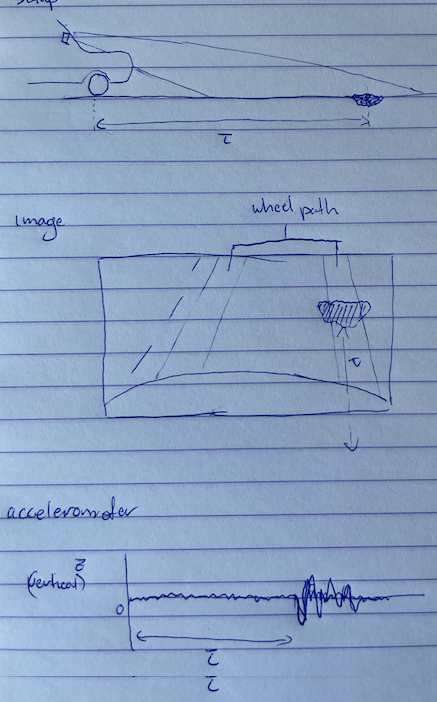
\includegraphics[height=18cm,keepaspectratio]{images/2_literature/sensor-delay.png}
\end{center}
\caption{Visualization of the sensor delay between measuring a defect. Top figure presents the setup. Middle shows the image data. Bottom shows the accelerometer data in the vertical Z-axes.\\TODO: Make it pretty}
\label{fig:sensor-delay}
\end{figure}


% When there is a similarity between the two data modalities, it is possible to align both streams 

% Cross correlation is a measure of similarity of two series as a function of the shift of one to the other.

% Learning from data often depends on cross correlation ...




% \subsection{Depth Estimation}




% The next challenge is that while driving, 

% The other method is to rely on 

% \textbf{Cross correlation}



% They use optical flow to capture fast ego-motion (i.e. vibration) for the front camera, and synchronize it with data from the accelerometer using cross correlation.

% One populair technique is Dynamic Time Warping (DTW). DTW measures the similarity between two sequences and finds the optimal match and inserts frames to align the time series.


% Most approaches to overcome this rely on a similarity measure between the modalities.  To overcome this, most approaches 



% \textbf{Cross correlation}

% \textbf{Dynamic Time Warping}

% \textbf{External trigger}
% One method to overcome this issue is using an external trigger to align the modalities. For instance in \cite{Cippitelli2015}, the authors are able to time synchronize visual data by calculating the delay when a controlled trigger is visible. 


% \subsection{Partial Observability}





% https://www.coursera.org/lecture/state-estimation-localization-self-driving-cars/lesson-2-multisensor-fusion-for-state-estimation-2imn3
















